\documentclass[UTF8, 12pt]{ctexart}
\usepackage{amsmath}
\usepackage{graphicx}
\usepackage{balance}
\usepackage{geometry}
\usepackage{fancyhdr}
\usepackage{amsthm}  
\usepackage[center]{titlesec}
\usepackage{color}
\usepackage{xcolor}
\usepackage{enumitem}
\usepackage{subfigure}
\usepackage{float}
%\usepackage{sectsty}
\usepackage[colorlinks,linkcolor=blue]{hyperref}


%页边距
\geometry{papersize={21cm,29.7cm}}
\geometry{left=1.18cm,right=1.18cm,top=2.54cm,bottom=2.54cm}

%\balance
%页眉页脚
\pagestyle{fancy}
\lhead{\title}
\cfoot{\thepage}
\renewcommand{\headrulewidth}{0.4pt}
\renewcommand{\headwidth}{\textwidth}
\renewcommand{\footrulewidth}{0pt}
%\sectionfont{\bfseries\raggedright}
%\setenumerate[1]{itemsep=0pt,partopsep=0pt,parsep=\parskip,topsep=5pt}
%\setitemize[1]{itemsep=0pt,partopsep=0pt,parsep=\parskip,topsep=5pt}

%段间距
\addtolength{\parskip}{.4em}
\graphicspath{{figures/}}


\author{金佳琪\\
\\
\large 中科院计算技术研究所}

\title{Onegis Web服务接口文档\_v0.6}
\date{\today}
 
%\makeatletter
%\renewcommand{\maketitle}{
%   \begin{titlepage}
%	 \vspace{5cm}
%     \begin{center}
%       \large
%       {\LARGE\@title}
%       \par\vspace{1ex}
%       \begin{tabular}[t]{c}
%         \@author
%       \end{tabular}
%       \vfill
%       \@date
%     \end{center}
%     \@thanks
%   \end{titlepage}
%}
%\makeatother

\begin{document}
\maketitle\thispagestyle{fancy}
\tableofcontents\thispagestyle{fancy}

\section{服务部署情况}
	Web服务部署在苏州服务器,使用PG Restful API进行开发。相关参数/部署情况/文档如下:
	\begin{table}[H]
		\centering
		\caption{查询接口及功能描述}
		\begin{tabular}{|p{6cm}|p{8cm}|}
			\hline
			参数名称 & 参数值 \\
			\hline
			本文档版本说明 & 版本为v0.6。基于新交换格式做了大量修改 \\
			\hline
			IP & 10.17.18.46 \\
			\hline
			Port & 8080 \\
			\hline
			数据库版本 & stodb1122 \\
			\hline
			数据库文档版本 & 多粒度对象数据库设计-2019-02-22.doc \\
			\hline
			JAVA jdk & 1.8 \\
			\hline
		\end{tabular}
	\end{table}

	\begin{table}[H]
		\centering
		\caption{接口完成情况}
		\begin{tabular}{|p{1cm}|p{6cm}|p{8cm}|}
			\hline
			序号 & 接口功能 & 完成情况 \\
			\hline
			1 & 基于id、name查询对象八元组 & 完成 \\
			\hline
			2 & 基于id、name列表作时空操作查询对象八元组 & 完成 \\
			\hline
			3 & 根据关系类型、关系递归深度查询相关对象 & 完成 \\
			\hline
			4 & 时空域查询 & 完成 \\
			\hline
			5 & 全生命周期查询、插入 & 查询包括在接口2功能中,插入暂缓 \\
			\hline
			6 & 父子对象查询 & parent与compose字段为空 \\
			\hline
			7 & 针对对象几个方面的修改 & 同插入,暂缓,后续版本提供 \\
			\hline
			8 & 时空缓冲区 & 功能整合到接口2中,查询的是position的位置 \\
			\hline
		\end{tabular}
	\end{table}
	
\section{多粒度时空对象查询接口}
\subsection{对象基本信息查询接口}
	\paragraph{接口参数}
		\begin{itemize}
			\item id: 对象id 可以为列表,逗号或空格分割
			\item sdomain 时空域id
			\item name: 对象名称 可以为列表,逗号或空格分隔
			\item begintime: 起始时间
			\item endtime: 结束时间
			\item wkt: 空间对象
			\item trs: 时间参照
			\item srs: 空间参照
			\item tuples: 八元组(attribute,form,attribute,model,compose,$\codts$) 逗号分隔,输出有对应字符的元组,不输入tuples默认为输出全部八元组
		\end{itemize}
	\paragraph{接口}
		接口形式如下:
		\newline
		{\color{red}/api/read/object/parm1/\{parm1\}/parm2/\{parm2\}$\cdots$}
		可用的参数组合及功能描述如下表所示
		\begin{table}[H]
			\centering
			\caption{查询接口及功能描述}
			\begin{tabular}{|p{6cm}|p{8cm}|}
				\hline
				功能 & 接口参数(按顺序) \\
				\hline
				根据对象时空域查 & sdomain \\
				\hline
				根据对象id查 & id \\
				\hline
				根据对象name查 & name \\
				\hline
				根据对象id及name查 & id, name \\
				\hline
				根据对象id列表作时空查询 & id,begintime,endtime,wkt,trs,srs \\
				\hline
				根据对象name列表作时空查询 & name,begintime,endtime,wkt,trs,srs \\
				\hline
				根据对象id及name列表作时空查询 & id, name, begintime,endtime,wkt,trs,srs \\
				\hline
			\end{tabular}
		\end{table}

	\paragraph{返回值说明}
		同交换格式对象
	\paragraph{查询示例}
		查询结果集 \\
		查询api\_1:【10.17.18.46:8080/api/read/object/sdomain/8939901214720】 \\
		查询api\_2:【10.17.18.46:8080/api/read/object/id/7849140314112】 \\
		查询api\_3:【10.17.18.46:8080/api/read/object/name/走廊/tuples/form】 \\
		查询api\_4:【10.17.18.46:8080/api/read/object/id/4094382637056, 7805735124992/name/路灯/begintime/1547110058000/endtime/1547110058001/wkt/POINT(114.2878191475 9.7140986105)/trs/1/srs/1】 \\
		下图仅作示例,非完整查询结果 \\
		{\color{red}注: 如果时间区间没有查询结果,返回对象版本中vtime<=begintime且最大的结果,如果仍无结果,不返回}
		\begin{figure}[H]
			\centering
			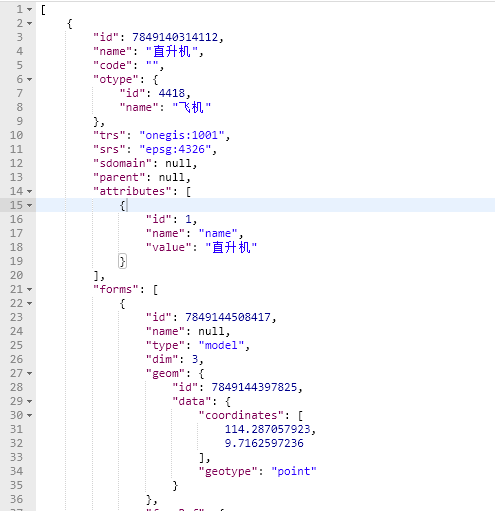
\includegraphics[width = 0.7\linewidth]{object.png}
			\caption{对象信息结果集}
			\label{Fig:1}
			\vspace{-0.5cm}
		\end{figure}

\subsection{关系查询接口}
	\paragraph{接口参数}
		\begin{itemize}
			\item id: 对象id
			\item dep: 递归层数
		\end{itemize}
	\paragraph{接口}
		接口形式如下:
		\newline
		{\color{red}/api/read/id/\{id\}/dep/\{dep\}}
	\paragraph{返回值说明}
		见查询示例

	\paragraph{查询示例}
		查询结果集 \\
		查询api:【10.17.18.46:8080/api/read/relation/id/1089800228745383936/dep/1】 \\
		下图仅作示例,非完整查询结果 \\
		\begin{figure}[H]
			\centering
			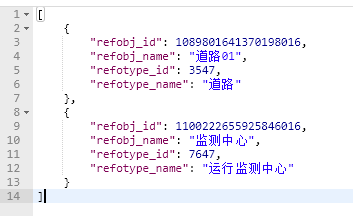
\includegraphics[width = 0.7\linewidth]{relation.png}
			\caption{关系结果集}
			\label{Fig:2}
			\vspace{-0.5cm}
		\end{figure}


%\subsection{形态信息查询接口}
%	\paragraph{接口参数}
%		\begin{itemize}
%			\item id: 对象id
%			\item timefilter: 时间,查询在指定时刻存活的对象,格式【yyyy-mm-dd hh:mm:ss.xxxxxx】
%		\end{itemize}
%	\paragraph{接口}
%		接口形式如下:
%		\newline
%		{\color{red}/api/form/parm1/\{parm1\}/parm2/\{parm2\}$\cdots$}
%		可用的参数组合及功能描述如下表所示
%		\begin{table}[H]
%			\centering
%			\caption{查询接口及功能描述}
%			\begin{tabular}{|p{6cm}|p{8cm}|}
%				\hline
%				功能 & 接口参数(按顺序) \\
%				\hline
%				根据对象id查 & id \\
%				\hline
%				根据对象id及时间查(对象不通时刻有不通的form) & id, timefilter \\
%				\hline
%			\end{tabular}
%		\end{table}
%
%
%	\paragraph{返回值说明}
%		如下
%		\begin{table}[H]
%			\centering
%			\caption{form返回值说明}
%			\begin{tabular}{p{3.5cm}|p{7cm}}
%				\hline
%				返回值 & 注释 \\
%				\hline
%				form\_id & 形态id \\
%				object\_id & 对象id \\
%				name & 形态名称 \\
%				time & 时间,如果没有,以part的时间为准 \\
%				state & 状态,如白天 \\
%				scale & 尺度,比例尺等 \\
%				srsid & \\
%				trsid & \\
%				locationdependence & 布尔值,true时使用模型坐标系,false时表示独立于位置进行形态描述 \\
%				formpart\_cur & 形态组成部分,见表~\ref{tab:formpart} \\
%				\hline
%			\end{tabular}
%		\end{table}
%
%		\begin{table}[H]
%			\centering
%			\caption{formpart返回值说明}
%			\label{tab:formpart}
%			\begin{tabular}{p{3.5cm}|p{7cm}}
%				\hline
%				返回值 & 注释 \\
%				\hline
%				formpart\_id & \\
%				form\_id & 属性id \\
%				name &  \\
%				type & 类型,如矢量、场 \\
%				shape & 形态 \\
%				dataformat & 组成部分数据格式,如JPG, 3DMAX \\
%				url &  \\
%				translation & 由此往后的参数(transform $\cdots$ q),描述空间形态与组成部分之间的位置和姿态变换 \\
%				transform &  \\
%				rotate &  \\
%				scale &  \\
%				geocoord &  \\
%				matrix &  \\
%				q &  \\
%				formpart\_parm\_cur & 参数信息,见表~\ref{tab:formparm} \\
%				formpart\_vec\_cur & 矢量信息,见表~\ref{tab:formvec} \\
%				formpart\_raster\_cur & 栅格信息,见表~\ref{tab:formraster} \\
%				formpart\_other\_cur & 其它信息,见表~\ref{tab:formother} \\
%				\hline
%			\end{tabular}
%		\end{table}
%
%		\begin{table}[H]
%			\centering
%			\caption{formpartparm返回值说明}
%			\label{tab:formparm}
%			\begin{tabular}{cc}
%				\hline
%				返回值 & 注释 \\
%				\hline
%				id & \\
%				formpart\_id \\
%				name & \\
%				valuetype & \\
%				value & \\
%				\hline
%			\end{tabular}
%		\end{table}
%
%		\begin{table}[H]
%			\centering
%			\caption{formpartvec返回值说明}
%			\label{tab:formvec}
%			\begin{tabular}{cc}
%				\hline
%				返回值 & 注释 \\
%				\hline
%				id & \\
%				formpart\_id & \\
%				vtime & 时间 \\ 
%				num & 节点数组(矢量数据节点) \\
%				vdata & \\
%				\hline
%			\end{tabular}
%		\end{table}
%
%		\begin{table}[H]
%			\centering
%			\caption{formpartraster返回值说明}
%			\label{tab:formraster}
%			\begin{tabular}{cc}
%				\hline
%				返回值 & 注释 \\
%				\hline
%				id & \\
%				formpart\_id & \\
%				metadata & 元数据xml \\
%				data & \\
%				\hline
%			\end{tabular}
%		\end{table}
%
%		\begin{table}[H]
%			\centering
%			\caption{formpartother返回值说明}
%			\label{tab:formother}
%			\begin{tabular}{cc}
%				\hline
%				返回值 & 注释 \\
%				\hline
%				id & \\
%				formpart\_id & \\
%				data & \\
%				\hline
%			\end{tabular}
%		\end{table}
%
%	\paragraph{查询示例}
%		查询结果集 \\
%		查询api:【ip:port/api/form/id/12372/timefilter/2018-09-08 00:00:00】 \\
%		下图仅作示例,非完整查询结果 \\
%		\begin{figure}[H]
%			\centering
%			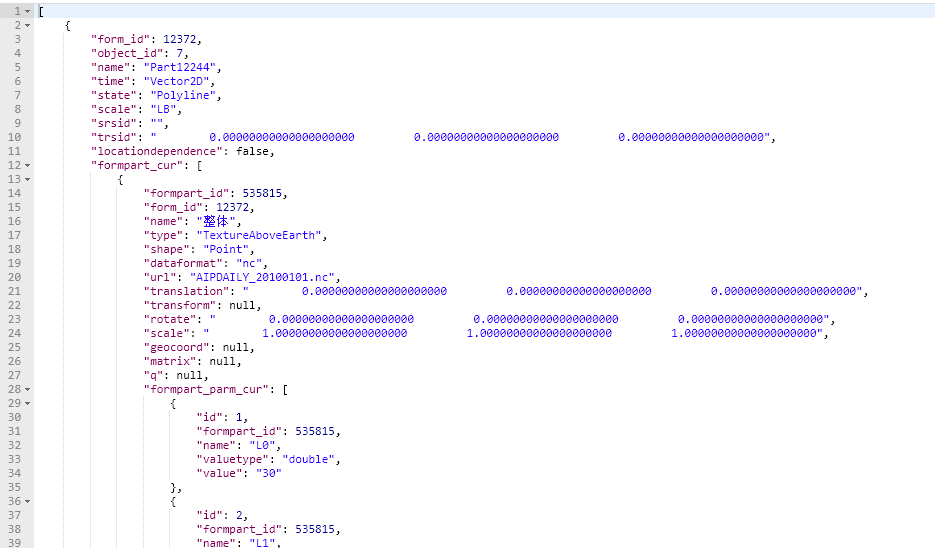
\includegraphics[width = 0.7\linewidth]{form.png}
%			\caption{形态信息结果集}
%			\label{Fig:3}
%			\vspace{-0.5cm}
%		\end{figure}
%
%
%\subsection{组成信息查询接口}
%	\paragraph{接口参数}
%		\begin{itemize}
%			\item id: 对象id
%		\end{itemize}
%	\paragraph{接口}
%		接口如下:
%		\newline
%		{\color{red}/api/part/id/\{id\}}
%
%	\paragraph{返回值说明}
%		如下
%		\begin{table}[H]
%			\centering
%			\caption{part返回值说明}
%			\begin{tabular}{cc}
%				\hline
%				返回值 & 注释 \\
%				\hline
%				partnotarrange\_cur & 组成部分非排列对象列表,见表~\ref{tab:partnotarr} \\
%				partarrange\_cur & 组成部分排列信息列表,见表~\ref{tab:partarr} \\
%				\hline
%			\end{tabular}
%		\end{table}
%
%		\begin{table}[H]
%			\centering
%			\caption{partnotarrange返回值说明}
%			\label{tab:partnotarr}
%			\begin{tabular}{cc}
%				\hline
%				返回值 & 注释 \\
%				\hline
%				id & \\
%				object\_id & \\
%				name & \\
%				refobjectid & 引用对象id \\
%				reftemplateid & 引用对象模板id \\
%				basecount & 不清楚 \\
%				translation & 由此往后的参数(transform $\cdots$ q),描述空间形态与组成部分之间\\的位置和姿态变换 \\
%				transform &  \\
%				rotate &  \\
%				scale &  \\
%				geocoord &  \\
%				matrix &  \\
%				q &  \\
%				\hline
%			\end{tabular}
%		\end{table}
%
%		\begin{table}[H]
%			\centering
%			\caption{partarrange返回值说明}
%			\label{tab:partarr}
%			\begin{tabular}{cc}
%				\hline
%				返回值 & 注释 \\
%				\hline
%				arrange\_id & \\
%				object\_id & \\
%				name & 排列名称名称 \\
%				type & M $\times$ N队列,三角形等 \\
%				translate & 整体与部分之间相对位置与姿态\\
%				partarrangeparm\_cur & 排列参数,见表~\ref{tab:arrangeparm} \\
%				partarrangeref\_cur & 排列引用,见表~\ref{tab:arrangeref} \\
%				\hline
%			\end{tabular}
%		\end{table}
%
%
%		\begin{table}[H]
%			\centering
%			\caption{partarrangeparm返回值说明}
%			\label{tab:arrangeparm}
%			\begin{tabular}{cc}
%				\hline
%				返回值 & 注释 \\
%				\hline
%				id & \\
%				partarrange\_id & \\
%				name & \\ 
%				valuetype & \\
%				value & \\
%				\hline
%			\end{tabular}
%		\end{table}
%
%		\begin{table}[H]
%			\centering
%			\caption{partarrangeref返回值说明}
%			\label{tab:arrangeref}
%			\begin{tabular}{cc}
%				\hline
%				返回值 & 注释 \\
%				\hline
%				id & \\
%				original\_id & 对象原始id \\
%				objecttemplate\_id & 对象模板id \\
%				objectfromgroup\_id & 对象所属集合 \\
%				istemplate & 是否为对象模板 \\
%				type & 对象类型 \\
%				name & 对象名称 \\
%				srsid & \\
%				trsid & \\
%				begintime & 对象初始化时间 \\
%				endtime & 对象消亡时间 \\
%				lifetime & 对象生命周期 \\
%				\hline
%			\end{tabular}
%		\end{table}
%
%	\paragraph{查询示例}
%		查询结果集 \\
%		查询api:【ip:port/api/part/id/1】 \\
%		目前数据库没有part信息 \\
%		\begin{figure}[H]
%			\centering
%			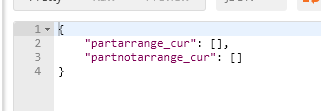
\includegraphics[width = 0.7\linewidth]{part.png}
%			\caption{组成信息结果集}
%			\label{Fig:4}
%			\vspace{-0.5cm}
%		\end{figure}
%
%
%\subsection{时空参照信息查询接口}
%	\paragraph{接口参数}
%		\begin{itemize}
%			\item id: 对象id
%		\end{itemize}
%	\paragraph{接口}
%		接口如下:
%		\newline
%		{\color{red}/api/srstrs/id/\{id\}}
%
%	\paragraph{返回值说明}
%		如下
%		\begin{table}[H]
%			\centering
%			\caption{srstrs返回值说明}
%			\label{tab:srstrs}
%			\begin{tabular}{cc}
%				\hline
%				返回值 & 注释 \\
%				\hline
%				objid & 对象id \\
%				srs\_id & 空间参照id \\
%				srs\_alias & 空间参照别名 \\
%				srs\_type & 空间参照类型 \\
%				srs\_vs & 空间参照描述字符串 \\
%				trs\_id & 时间参照id \\
%				trs\_alias & 时间参照别名 \\
%				trs\_type & 时间参照类型 \\
%				trs\_vs & 时间参照描述字符串 \\
%				\hline
%			\end{tabular}
%		\end{table}
%
%	\paragraph{查询示例}
%		查询结果集 \\
%		查询api:【ip:port/api/srstrs/id/1】 \\
%		目前数据库没有自定义时空参照信息 \\
%		%\begin{figure}[H]
%		%	\centering
%		%	\includegraphics[width = 0.7\linewidth]{srstrs.png}
%		%	\caption{时空参照信息结果集}
%		%	\label{Fig:5}
%		%	\vspace{-0.5cm}
%		%\end{figure}
%
%
%\subsection{位置信息查询接口}
%	\paragraph{接口参数}
%		\begin{itemize}
%			\item id: 对象id
%			\item timefilter: 时间,查询在指定时刻存活的对象,格式【yyyy-mm-dd hh:mm:ss.xxxxxx】
%		\end{itemize}
%	\paragraph{接口}
%		接口形式如下:
%		\newline
%		{\color{red}/api/position/parm1/\{parm1\}/parm2/\{parm2\}$\cdots$}
%		可用的参数组合及功能描述如下表所示
%		\begin{table}[H]
%			\centering
%			\caption{查询接口及功能描述}
%			\begin{tabular}{|p{6cm}|p{8cm}|}
%				\hline
%				功能 & 接口参数(按顺序) \\
%				\hline
%				根据对象id查 & id \\
%				\hline
%				根据对象id及时间查(对象有动态位置及实时位置) & id, timefilter \\
%				\hline
%			\end{tabular}
%		\end{table}
%
%	\paragraph{返回值说明}
%		\begin{table}[H]
%			\centering
%			\caption{position返回值说明}
%			\label{tab:postion}
%			\begin{tabular}{cc}
%				\hline
%				返回值 & 注释 \\
%				\hline
%				pos\_id & \\
%				object\_id & \\
%				pos\_type & 位置类型,静态、动态、实时、函数、轨道等 \\
%				pos\_shape & 位置的形状 \\
%				pos\_format & 数据格式,XY,BL,XYZ等\\
%				srsid &  \\
%				trsid &  \\
%				posparm\_cur & 位置参数,见表~\ref{tab:posparm} \\
%				stadym\_cur & 动态、静态位置参数,见表~\ref{tab:posdym} \\
%				real\_cur & 实时位置,见表~\ref{tab:posreal} \\
%				fun\_cur & 函数位置,见表~\ref{tab:posfunc} \\
%				orbit\_cur & 轨道位置,见表~\ref{tab:posorbit} \\
%				\hline
%			\end{tabular}
%		\end{table}
%
%		\begin{table}[H]
%			\centering
%			\caption{posparm返回值说明}
%			\label{tab:posparm}
%			\begin{tabular}{cc}
%				\hline
%				返回值 & 注释 \\
%				\hline
%				parm\_id & \\
%				pos\_id & position表id \\
%				parm\_name & 参数名称\\
%				parm\_valuetype & \\
%				parm\_value & \\
%				\hline
%			\end{tabular}
%		\end{table}
%
%		\begin{table}[H]
%			\centering
%			\caption{posdym返回值说明}
%			\label{tab:posdym}
%			\begin{tabular}{cc}
%				\hline
%				返回值 & 注释 \\
%				\hline
%				stadym\_id & \\
%				pos\_id & position表id \\
%				dym\_time & 时间 \\
%				num & 对应矢量数据节点数组 \\
%				stadym\_data & \\
%				\hline
%			\end{tabular}
%		\end{table}
%		
%		\begin{table}[H]
%			\centering
%			\caption{posreal返回值说明}
%			\label{tab:posreal}
%			\begin{tabular}{cc}
%				\hline
%				返回值 & 注释 \\
%				\hline
%				pos\_id & position表id \\
%				real\_time & 时间 \\
%				real\_location & 实时位置,流数据 \\
%				datalength & \\
%				\hline
%			\end{tabular}
%		\end{table}
%
%		\begin{table}[H]
%			\centering
%			\caption{posfunction返回值说明}
%			\label{tab:posfunc}
%			\begin{tabular}{cc}
%				\hline
%				返回值 & 注释 \\
%				\hline
%				func\_id & \\
%				pos\_id & position表id \\
%				func\_data & \\
%				\hline
%			\end{tabular}
%		\end{table}
%
%		\begin{table}[H]
%			\centering
%			\caption{posorbit返回值说明}
%			\label{tab:posorbit}
%			\begin{tabular}{cc}
%				\hline
%				返回值 & 注释 \\
%				\hline
%				orbit\_id &  \\
%				pos\_id & position表id \\
%				orbit\_type & \\
%				\hline
%			\end{tabular}
%		\end{table}
%
%	\paragraph{查询示例}
%		查询结果集 \\
%		查询api:【ip:port/api/position/id/1/timefilter/2018-11-09 09:34:58.0】 \\
%		\begin{figure}[H]
%			\centering
%			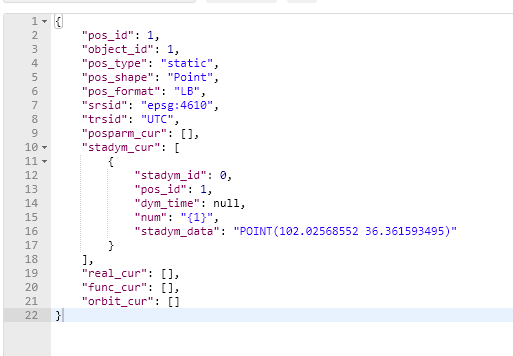
\includegraphics[width = 0.7\linewidth]{position.png}
%			\caption{位置信息结果集}
%			\label{Fig:6}
%			\vspace{-0.5cm}
%		\end{figure}
%
%\subsection{对象行为信息查询接口}
%	\paragraph{接口参数}
%		\begin{itemize}
%			\item id: 对象id
%		\end{itemize}
%	\paragraph{接口}
%		接口如下:
%		\newline
%		{\color{red}/api/srstrs/id/\{id\}}
%
%	\paragraph{返回值说明}
%		如下
%		\begin{table}[H]
%			\centering
%			\caption{action返回值说明}
%			\label{tab:action}
%			\begin{tabular}{cc}
%				\hline
%				返回值 & 注释 \\
%				\hline
%				action\_id & 行为id \\
%				object\_id & \\
%				name & \\
%				type & \\
%				trigger & 行为触发方式\\
%				triggerparameter & 行为触发参数 \\
%				result & 行为结果 \\
%				actionparm\_cur & 行为参数,见表~\ref{tab:actionparm} \\
%				actionlifetime\_cur & 行为生命周期,见表~\ref{tab:actionlife} \\
%				actionpath\_cur & 行为路径,见表~\ref{tab:actionpath} \\
%				\hline
%			\end{tabular}
%		\end{table}
%
%		\begin{table}[H]
%			\centering
%			\caption{actionparm返回值说明}
%			\label{tab:actionparm}
%			\begin{tabular}{cc}
%				\hline
%				返回值 & 注释 \\
%				\hline
%				id & \\
%				objectaction\_id & \\
%				name & \\
%				valuetype & \\
%				value & \\
%				\hline
%			\end{tabular}
%		\end{table}
%
%		\begin{table}[H]
%			\centering
%			\caption{actionlifetime返回值说明}
%			\label{tab:actionlife}
%			\begin{tabular}{cc}
%				\hline
%				返回值 & 注释 \\
%				\hline
%				id & \\
%				objectaction\_id & \\
%				trsid & \\
%				begintime & \\
%				endtime & \\
%				lifetime & \\
%				\hline
%			\end{tabular}
%		\end{table}
%
%		\begin{table}[H]
%			\centering
%			\caption{actionpath返回值说明}
%			\label{tab:actionpath}
%			\begin{tabular}{cc}
%				\hline
%				返回值 & 注释 \\
%				\hline
%				id & \\
%				objectaction\_id & \\
%				srsid & \\
%				needsmooth & 是否需要平滑 \\
%				interpointsnum & 插值点数 \\
%				constantspeed & 是否匀速 \\
%				shape & 抽样点形状,通常是POINT \\
%				format & 数据格式,XY/XYZ/LB/LBH等 \\
%				url & 资源路径信息 \\
%				pathdata\_cur & 路径数据列表,见表~\ref{tab:pathdata} \\
%				\hline
%			\end{tabular}
%		\end{table}
%
%		\begin{table}[H]
%			\centering
%			\caption{actionpathdata返回值说明}
%			\label{tab:pathdata}
%			\begin{tabular}{cc}
%				\hline
%				返回值 & 注释 \\
%				\hline
%				id & \\
%				path\_id & \\
%				time & \\
%				num & \\
%				data & \\
%				\hline
%			\end{tabular}
%		\end{table}
%
%	\paragraph{查询示例}
%		查询结果集 \\
%		查询api:【ip:port/api/action/id/29770】 \\
%		连续轨迹数据
%		\begin{figure}[H]
%			\centering
%			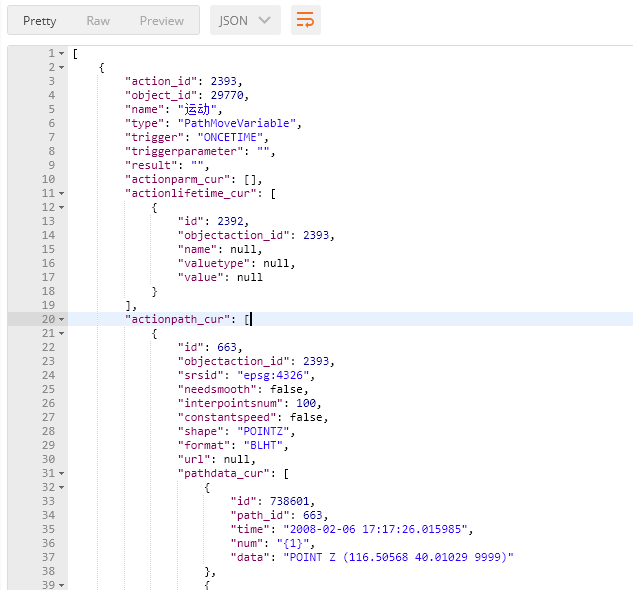
\includegraphics[width = 0.7\linewidth]{action.png}
%			\caption{行为信息结果集}
%			\label{Fig:action}
%			\vspace{-0.5cm}
%		\end{figure}
%
%\subsection{根据id和时间获取对象全部信息}
%	\paragraph{接口参数}
%		\begin{itemize}
%			\item id: 对象id
%			\item timefilter: 时间,查询在指定时刻存活的对象,格式【yyyy-mm-dd hh:mm:ss.xxxxxx】
%		\end{itemize}
%	\paragraph{接口}
%		接口如下:
%		\newline
%		{\color{red}/api/all/id/\{id\}/timefilter/\{time\}}
%
%	\paragraph{返回值说明}
%		本节前述所有内容(除action)组合即为一个对象的全部信息
%
%	\paragraph{查询示例}
%		查询结果集 \\
%		查询api:【ip:port/api/position/id/2761/timefilter/2018-11-09 09:34:58.0】 \\
%		\begin{figure}[H]
%			\centering
%			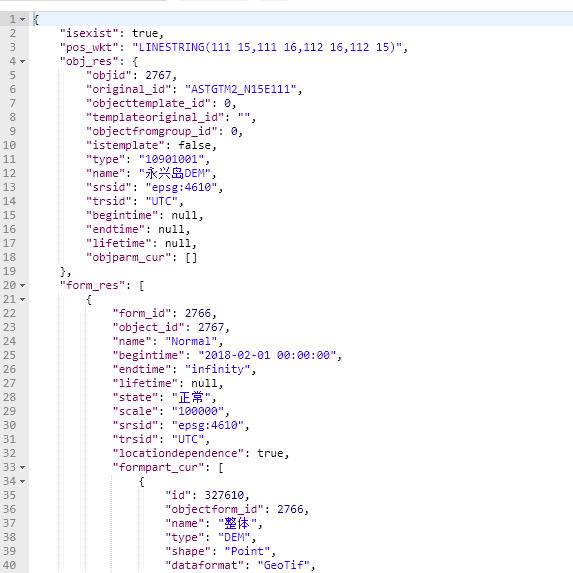
\includegraphics[width = 0.7\linewidth]{all.png}
%			\caption{对象完整信息结果集}
%			\label{Fig:6}
%			\vspace{-0.5cm}
%		\end{figure}
%
%\section{基本功能函数}
%	
%\subsection{获取所有对象基本信息}
%	\paragraph{接口参数}
%		无参数,本接口用于获取对象的基本信息(id, name)
%	\paragraph{接口}
%		接口如下:
%		\newline
%		{\color{red}/api/feature/baseinfo}
%
%	\paragraph{查询示例}
%		查询结果集 \\
%		查询api:【ip:port/api/features/baseinfo】 \\
%		\begin{figure}[H]
%			\centering
%			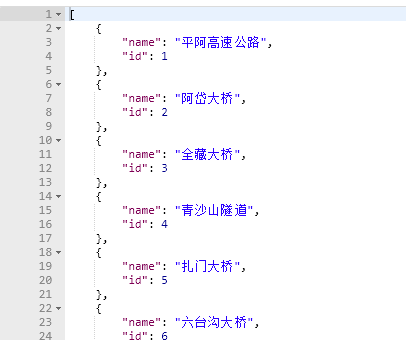
\includegraphics[width = 0.7\linewidth]{baseinfo.png}
%			\caption{对象基本信息结果集}
%			\label{Fig:7}
%			\vspace{-0.5cm}
%		\end{figure}
%
%\subsection{获取子对象id}
%	\paragraph{接口参数}
%		\begin{itemize}
%			\item id: 当前对象id
%		\end{itemize}
%	\paragraph{接口}
%		接口如下:
%		\newline
%		{\color{red}/api/feature/subobjid/id/\{id\}}
%
%	\paragraph{查询示例}
%		查询结果集 \\
%		查询api:【ip:port/api/features/subobjid/id/1】 \\
%		子对象获取借助八元组-Part。目前无Part数据,因此本接口无法获取结果 \\
%		%\begin{figure}[H]
%		%	\centering
%		%	\includegraphics[width = 0.7\linewidth]{subobj.png}
%		%	\caption{子对象id信息结果集}
%		%	\label{Fig:8}
%		%	\vspace{-0.5cm}
%		%\end{figure}
%
%\subsection{获取父对象id}
%	\paragraph{接口参数}
%		\begin{itemize}
%			\item id: 当前对象id
%		\end{itemize}
%	\paragraph{接口}
%		接口如下:
%		\newline
%		{\color{red}/api/feature/parobjid/id/\{id\}}
%
%	\paragraph{查询示例}
%		查询结果集 \\
%		查询api:【ip:port/api/features/parobjid/id/1】 \\
%		父对象获取借助八元组-Part。目前无Part数据,因此本接口无法获取结果 \\
%		%\begin{figure}[H]
%		%	\centering
%		%	\includegraphics[width = 0.7\linewidth]{parobj.png}
%		%	\caption{父对象id信息结果集}
%		%	\label{Fig:9}
%		%	\vspace{-0.5cm}
%		%\end{figure}
%
%\subsection{获取对象id(分页+时间)}
%	\paragraph{接口参数}
%		\begin{itemize}
%			\item pageNum: 页码
%			\item pageSize: 页大小
%			\item timefilter: 时间,查询在指定时刻存活的对象,格式【yyyy-mm-dd hh:mm:ss.xxxxxx】
%		\end{itemize}
%	\paragraph{接口}
%		接口如下:
%		\newline
%		{\color{red}/api/feature/objid/parm1/\{parm1\}/parm2/\{parm2\}$\cdots$}
%		可用的参数组合及功能描述如下表所示
%		\begin{table}[H]
%			\centering
%			\caption{查询接口及功能描述}
%			\begin{tabular}{|p{6cm}|p{8cm}|}
%				\hline
%				功能 & 接口参数(按顺序) \\
%				\hline
%				分页查 & pageNum, pageSize \\
%				\hline
%				分页+时间查(对象有存活时间) & pageNum, pageSize, timefilter \\
%				\hline
%			\end{tabular}
%		\end{table}
%
%	\paragraph{查询示例}
%		查询结果集 \\
%		查询api:【ip:port/api/features/objid/pageNum/1/pageSize/10/timefilter/2008-01-20 00:00:00】 \\
%		\begin{figure}[H]
%			\centering
%			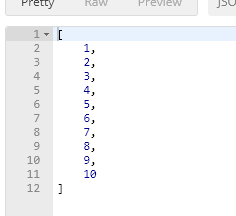
\includegraphics[width = 0.7\linewidth]{objid.png}
%			\caption{对象id信息结果集}
%			\label{Fig:10}
%			\vspace{-0.5cm}
%		\end{figure}
%
%\section{空间操作接口}
%
%\subsection{根据输入空间对象+时间返回对象id}
%	\paragraph{接口参数}
%		\begin{itemize}
%			\item wkt: 空间对象
%			\item srsid: 对象空间参照【如4610...】
%			\item time: 时间,需要根据指定时刻确定对象位置,格式【yyyy-mm-dd hh:mm:ss.xxxxxx】
%		\end{itemize}
%	\paragraph{接口}
%		接口如下:
%		\newline
%		{\color{red}/api/geom/op?wkt=\{wkt\}\&srsid=\{srsid\}\&time=\{time\}【op由具体操作类型替代】}
%		可用的操作接口及功能描述如下表所示
%		\begin{table}[H]
%			\centering
%			\caption{查询接口及功能描述}
%			\begin{tabular}{|p{6cm}|p{8cm}|}
%				\hline
%				功能 & 接口参数(按顺序) \\
%				\hline
%				判断对象与输入几何体是否分离 & disjoint \\
%				\hline
%				判断对象与输入几何体是否相交 & intersects \\
%				\hline
%				判断对象与输入几何体是否接触 & touches \\
%				\hline
%				判断对象与输入几何体是否交叉 & crosses \\
%				\hline
%				判断对象是否被输入几何体离包含 & contains \\
%				\hline
%				判断对象与输入几何体是否重叠 & overlaps \\
%				\hline
%				判断对象与输入几何体是否相同 & equals \\
%				\hline
%			\end{tabular}
%		\end{table}
%
%	\paragraph{查询示例}
%		查询结果集 \\
%		查询api:【ip:port/api/geom/disjoint?wkt=POINT(7 8)\&srsid=4610\&time=2018-10-1 00:00:00】 \\
%		\begin{figure}[H]
%			\centering
%			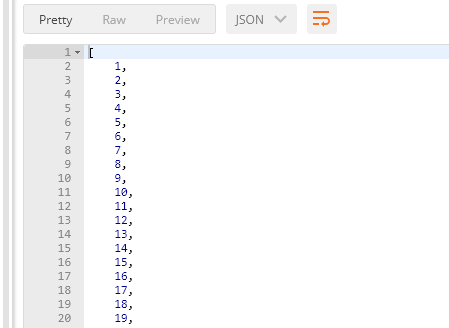
\includegraphics[width = 0.7\linewidth]{geom_op.png}
%			\caption{空间查询(分离disjoint)结果集}
%			\label{Fig:11}
%			\vspace{-0.5cm}
%		\end{figure}
%
%
%\subsection{两个输入对象的空间关系查询}
%	\paragraph{接口参数}
%		\begin{itemize}
%			\item wkt1: 对象1
%			\item wkt2: 对象2
%			\item len: 距离(部分操作需要距离参数,如dwithin)
%		\end{itemize}
%	\paragraph{接口}
%		接口如下:
%		\newline
%	{\color{red}/api/spatial/op?parm1=\{parm1\}\&parm2=\{parm2\}$\cdots$【op由具体操作类型替代,部分接口需要len】}
%		可用的操作接口及功能描述如下表所示
%		\begin{table}[H]
%			\centering
%			\caption{查询接口及功能描述}
%			\begin{tabular}{|p{6cm}|p{8cm}|}
%				\hline
%				功能 & 接口参数(按顺序) \\
%				\hline
%				求两个对象的距离 & distance, wkt1, wkt2 \\
%				\hline
%				判断两个对象距离是否超出len & dwithin, wkt1, wkt2, len \\
%				\hline
%				判断两个对象是否相同 & equals, wkt1, wkt2 \\
%				\hline
%				判断两个对象是否分离 & disjoint, wkt1, wkt2 \\
%				\hline
%				判断两个对象是否相交 & intersects, wkt1, wkt2 \\
%				\hline
%				判断两个对象是否接触 & touches, wkt1, wkt2 \\
%				\hline
%				判断两个对象是否交叉 & crosses, wkt1, wkt2 \\
%				\hline
%				判断对象1是否包含对象2 & contains, wkt1, wkt2 \\
%				\hline
%				判断两个对象重叠 & overlaps, wkt1, wkt2 \\
%				\hline
%				判断对象1是否覆盖对象2 & covers, wkt1, wkt2 \\
%				\hline
%			\end{tabular}
%		\end{table}
%
%	\paragraph{查询示例}
%		查询结果集 \\
%		查询api\_1:【ip:port/api/spatial/dwithin?wkt1=Point(0 0)\&wkt2=Point(3 3)\&len=5.0】 \\
%		查询api\_2:【ip:port/api/spatial/distance?wkt1=Point(1 2)\&wkt2=Point(3 4)】 \\
%	\paragraph{返回值说明}
%		\begin{itemize}
%			\item distance: 返回距离
%			\item 其它: 返回1(True)或0(False)
%		\end{itemize}

\end{document}
